\chapter{Experimental Results}\label{ch:experimental_result}
In this chapter, we are going to evaluate our proposed method at different experimental setup on multiple benchmark datasets. In Section~\ref{sec:datasets}, we have explained different state-of-the-art gait recognition datasets that we used to train and evaluate our proposed method. As to estimate pose, RGB video frames are required, hence, we couldn't evaluate our method to those datasets which only consists of silhouette sequences.  In Section~\ref{sec:single_view} and Section~\ref{sec:cross_view} we have presented the experimental results of our proposed method on single-view and cross-view gait recognition respectively. The performance of our method in multi-view gait recognition is discussed in Section~\ref{sec:multi_view}.

%-------------------------------------------------------------------------
\section{Dataset} \label{sec:datasets}
The success of deep learning-based algorithms greatly depends on the vast amount of labeled training data. However, unfortunately, few existing gait datasets have a large number of subjects as well as a variety of covariate factors. Some of the publicly available gait datasets are CASIA A and CASIA B gait dataset~\cite{Yu_06}, TUM GAID dataset~\cite{Hofmann_14}, SOTON database~\cite{Shutler_04}, OU-ISIR multi-view large population dataset (OU-MVLP)~\cite{Noriko_18}, and USF HumanID dataset~\cite{Sarkar_05}. 

\begin{figure}
	\centering
	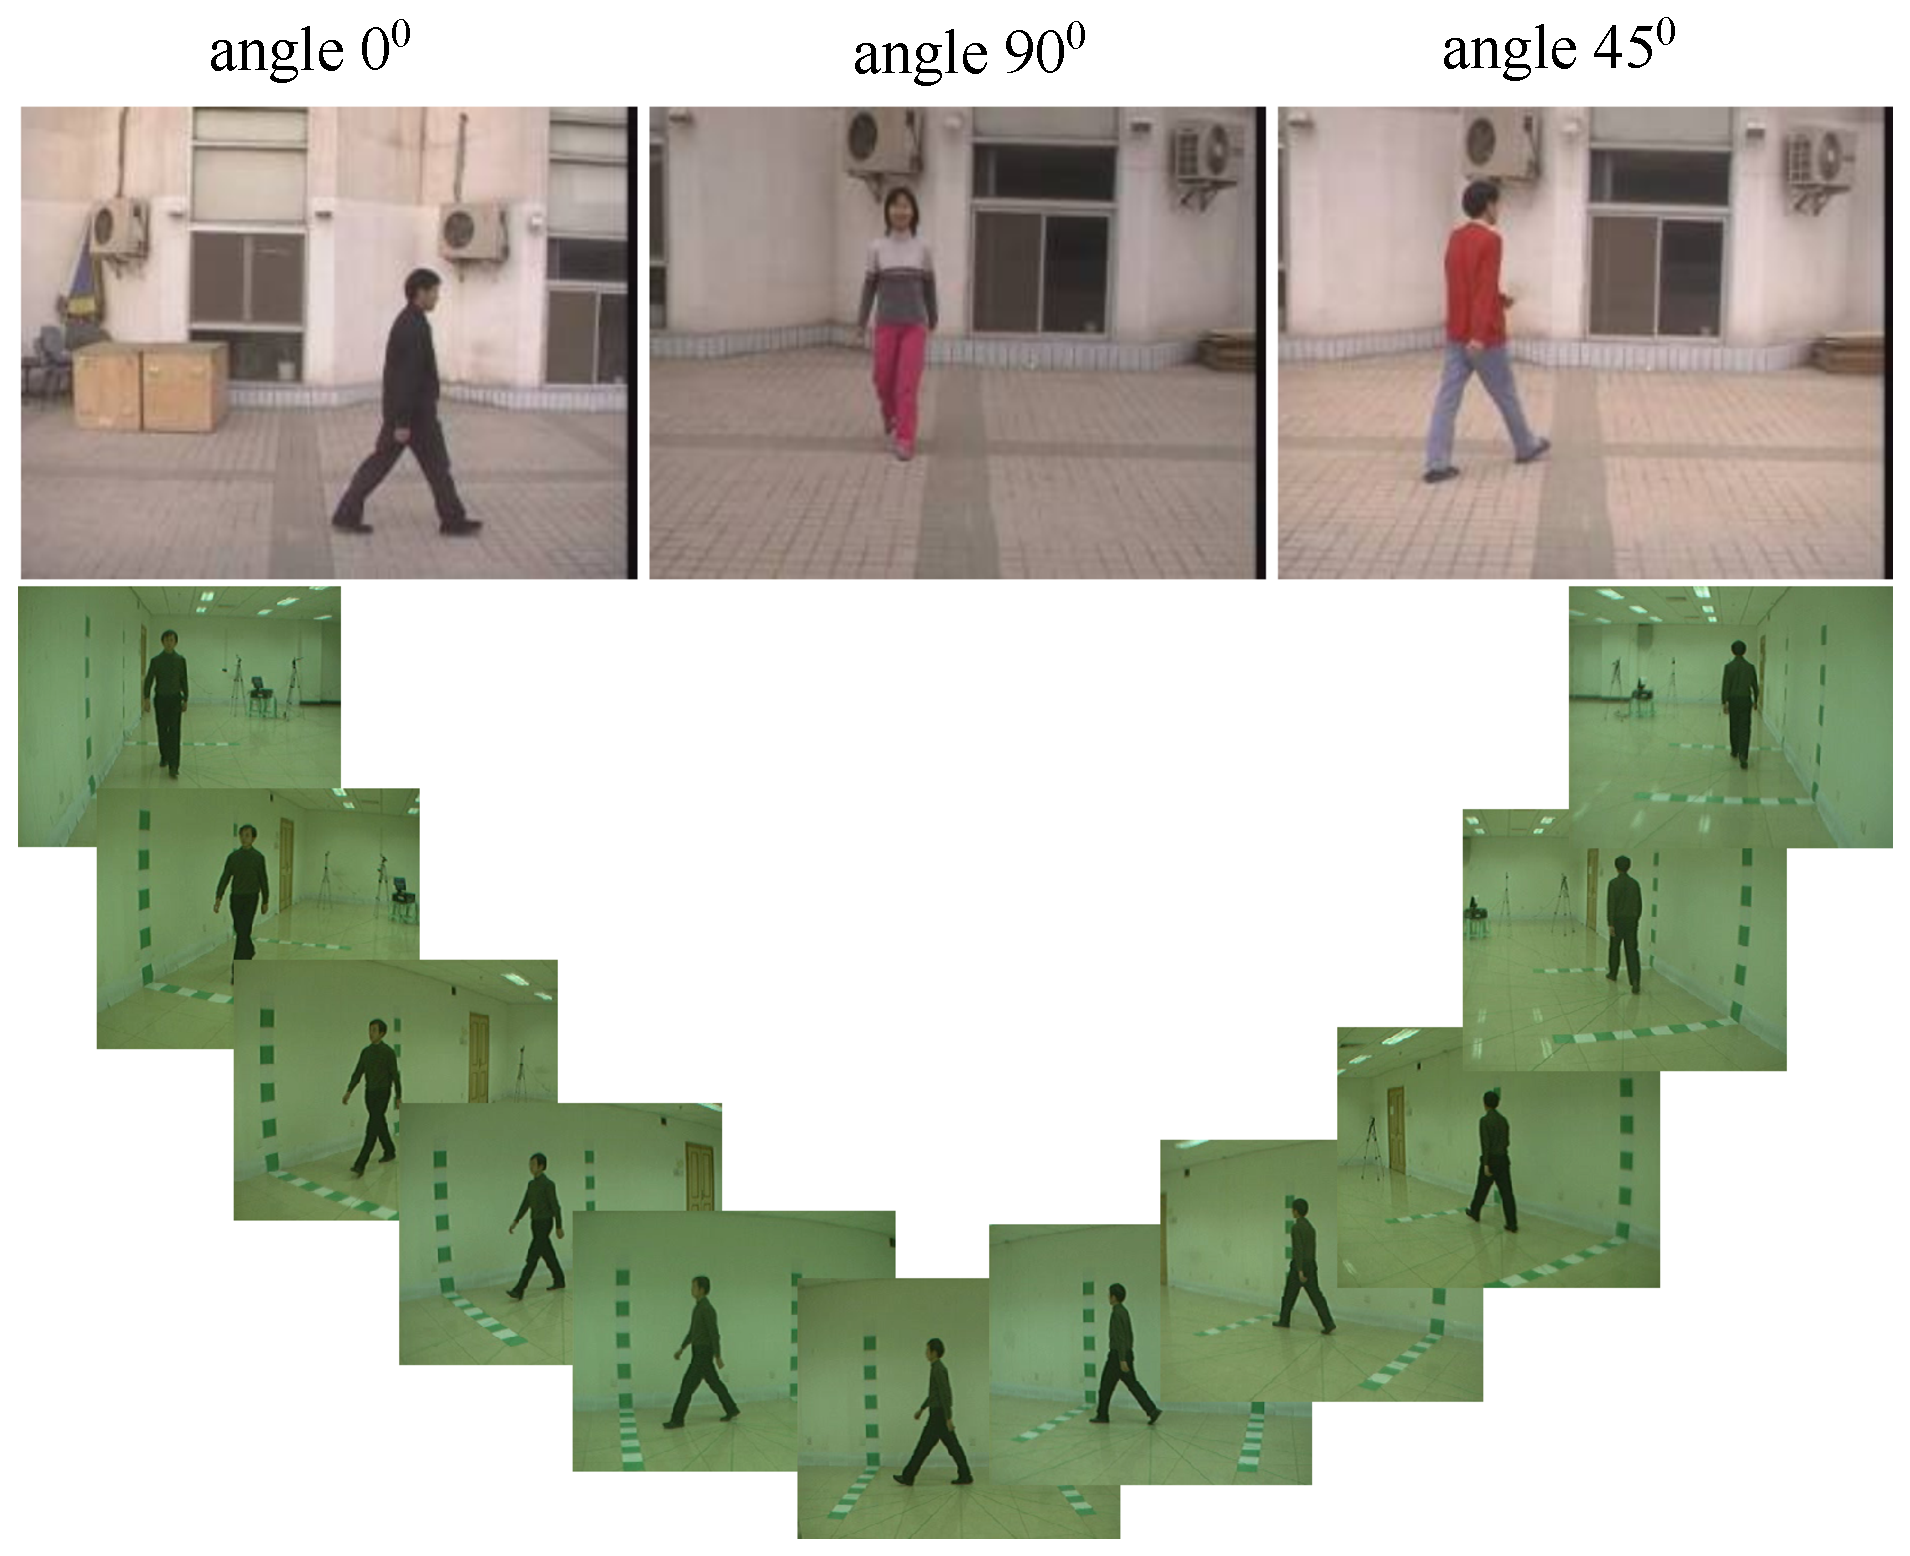
\includegraphics[width = 0.7\textwidth]{figures/casia_dataset.eps}
	\caption [Sample video frames of CASIA A and CASIA B dataset]
	{Sample video frames of CASIA A and CASIA B dataset. In top, some of the sample images from CASIA A dataset are shown where the subjects are walking along the straight line in $ 3 $ different view angles, and in bottom, CASIA B dataset is shown with its $ 11 $ view angles.
	}
	\label{fig:casia_dataset}
\end{figure} 

\begin{itemize}
	\item \textbf{USF HumanID gait dataset}~\cite{Sarkar_05}: there are $ 122 $ subjects walking outside on two different surfaces of an elliptical path under two different time, view angle, clothing, shoes, and carrying conditions. However, every subject was not filmed under all conditions.
	
	\item \textbf{TUM GAID dataset}~\cite{Hofmann_14}: Another large dataset for gait recognition which consists of $ 305 $ subjects where each subject has $ 10 $ gait videos. As, all of the videos were recorded from the side view angle, this dataset is not suitable for evaluating the performance on multi-view gait recognition.
	
	\item \textbf{CMU MoBo dataset}~\cite{Gross_01}: This dataset has $25$ subjects with six views and four walking styles. The main drawback of this database is that all the data is from an indoor environment (collected from a treadmill). Six cameras are positioned to cover the complete field-of-view of the walking person on the treadmill.
	
	\item \textbf{SOTON database}~\cite{Shutler_04}: It contains two types of datasets – a large dataset with more than 100 subjects and a small dataset with only 10 subjects. The large dataset has two viewpoints (frontal and oblique) and contains subjects in both outdoor and indoor environments and on a treadmill. The small database is used to explore gait recognition under covariates such as views, shoes, clothing, carriage, and walking speed.
	
	\item \textbf{OU-ISIR multi-view large population dataset (OU-MVLP)}~\cite{Noriko_18}: The largest dataset available for gait recognition. It contains $ 10,307 $ subjects from $ 14 $ view angles ranging from ${{0}^{\circ}-{90}^{\circ}}$, and ${{180}^{\circ}-{270}^{\circ}}$. Only two sequences are provided, one for the gallery and the other for the probe. But, this dataset is only formatted as a set of silhouette sequence which makes it completely different from our approach.
	
	\item \textbf{CASIA (CASIA A and CASIA B) dataset}~\cite{Yu_06}: one of the largest datasets for multi-view gait recognition. CASIA A dataset contains total $ 20 $ subjects walking in an outdoor environment where CASIA B dataset contains total $ 124 $ subjects walking in an indoor environment. In CASIA A gait dataset, each subject walks along a straight line in 3 different view angles: lateral (${0^{\circ}}$), oblique (${45^{\circ}}$), and frontal (${90^{\circ}}$). For each view angle all subjects have total four gait sequences out of which two of them have same walking direction while the other two have opposite direction. 
	
	In CASIA B dataset, there are 10 walking sequences for each subject: 6 sequences for normal walking ('nm'), 2 sequences for walking in coat ('cl') and 2 sequences for walking with bag ('bg') on shoulder. Therefore, this dataset separately considered three variations in people walking namely normal, clothing, and carrying condition. Also, each walking sequence were captured from 11 view angles ranging from ${0^{\circ}}$ to ${180^{\circ}}$. Figure~\ref{fig:casia_dataset} illustrates some of the sample video frames of CASIA A and CASIA B datasets.
\end{itemize}



\begin{figure}
	\centering
	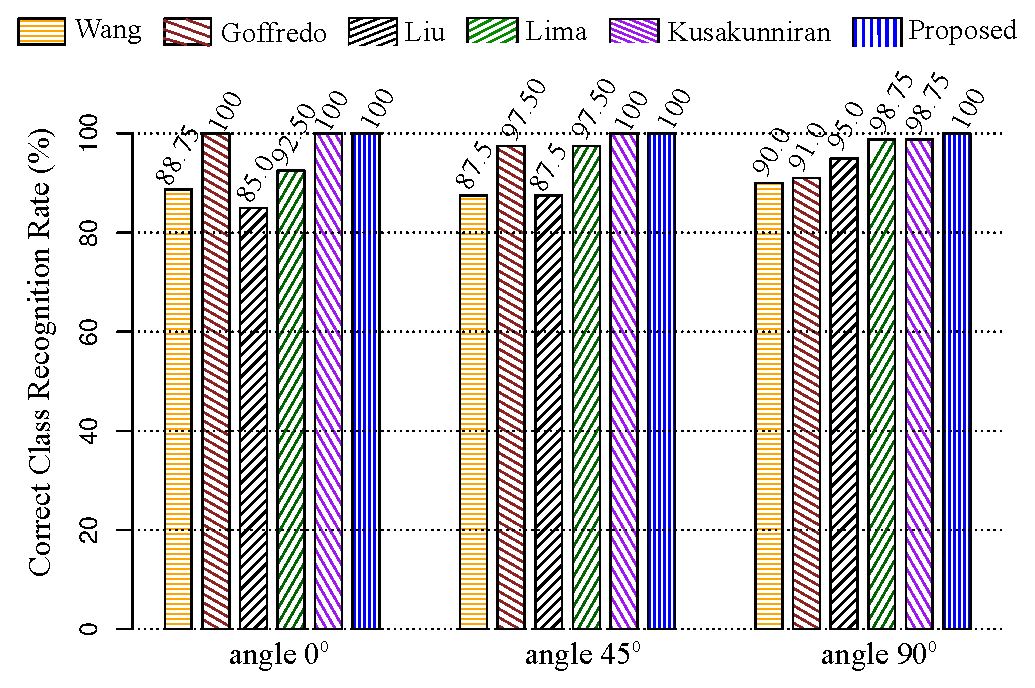
\includegraphics[width = 0.8\textwidth]{figures/casia_a_result.eps}
	\caption [Comparison in CCR among proposed method with other prevailing gait recognition methods at different view angles on CASIA A dataset]
	{Comparison in CCR among proposed method with other prevailing gait recognition methods at different view angles on CASIA A dataset. Our method achieves $ \textbf{100\% }$ CCR on all of the view angles which showed the efficacy of the proposed method. \label{fig:casia_a_result}
	}
	
\end{figure}

%-------------------------------------------------------------------------
\section{Single-View Gait Recognition} \label{sec:single_view}
\subsection{Experimental Evaluation on CASIA A dataset}
Since, CASIA A dataset contains only $ 20 $ subjects where every subject has only four gait sequences in three different view angles, we trained a model for each of the view angle with $ 20 $ output neurons in the final softmax layer of our proposed network. To evaluate the performance of our proposed method on CASIA A dataset, we employed leave-one-out cross validation rule, i.e., one sequence was set for testing and the remainder was set for training the network. We compare our results with five other prevailing state-of-the-art gait recognition methods including Wang~\cite{Wang_03}, Goffredo~\cite{Goffredo_08}, Liu~\cite{Liu_16}, Lima~\cite{Lima_19}, and Kusakunniran~\cite{Kusakunniran_09} (see Figure~\ref{fig:casia_a_result}). Table~\ref{table:casia_a_result} illustrates the comparison where it is seen that the proposed method have achieved higher average correct class recognition rates (\gls{ccr}) of $100.0\%$ compared to other methods in literature.


\begin{table}
	\centering
	\caption [Comparison among different state-of-the-art gait recognition methods without view variation in all three view angles of CASIA A dataset]
	{Comparison among different state-of-the-art gait recognition methods without view variation in all three view angles of CASIA A dataset. It has been observed that the proposed method achieves the highest average recognition rate, i.e., \textbf{100.0\%} on all three angles and outperforms other state-of-the-art methods by a large margin. \label{table:casia_a_result}}
	{\begin{tabular*}{30pc}{@{\extracolsep{\fill}}ccccc}\hline
			
			Methods &${0^{\circ}}$ &${45^{\circ}}$   &${90^{\circ}}$  &Mean\\
			\hline
			
			Wang~\cite{Wang_03} &88.75 &87.50 &90.00 &88.75\\
			
			\noalign{\smallskip}
			Goffredo~\cite{Goffredo_08} &100.0 &97.50 &91.00 &96.16\\ 
			
			\noalign{\smallskip}
			Liu~\cite{Liu_16} &85.00 &87.50 &95.00 &89.17\\ 
			
			\noalign{\smallskip}
			Lima~\cite{Lima_19} &92.50 &97.50 &98.75 &96.25 \\
			
			\noalign{\smallskip}
			Kusakunniran~\cite{Kusakunniran_09} &100  &100  &98.75 &99.58 \\
			
			\noalign{\smallskip}
			Proposed &{\textbf{100.0}} & {\textbf{100.0}} &{\textbf{100.0}} & {\textbf{100.0}}\\
			\hline
	\end{tabular*}}{}
\end{table}


\subsection{Experimental Evaluation on CASIA B Dataset}
\subsubsection{Experimental Setup}
We designed two experimental setups (A, B), as demonstrated in Table~\ref{table:caisab_setup}, for evaluating the performance in CASIA B dataset. Experimental setup A was for evaluating the performance of our proposed method in single-view gait recognition. To investigate the robustness of view variation, comparison results of the proposed method against other state-of-the-art methods in different view variations have been reported. Experiment setup B was designed for evaluating the cross-view recognition performance. 

For setup A,  we divided the dataset into two groups where the first group consists of 62 subjects which is used to train the network. The second group contains rest of the subjects for evaluating the performance of the network. For experimental setup B, the ratio between the train and evaluation set was 24 to 100. In the evaluation set for both setup, 4 normal walking sequences of each subject are put into gallery set and rest 6 walking sequences consist three probe set (\textit{ProbeNM}, \textit{ProbeBG}, \textit{ProbeCL}). \textit{ProbeNM} consists of 2 other normal walking sequences where \textit{ProbeBG} and \textit{ProbeCL} consist of two sequences of carrying bag and wearing coat respectively.

\begin{table}[t]
	\centering
	\caption[Experimental setup for the CASIA B dataset]
	{Experimental setup for the CASIA B dataset. The dataset was divided into two different setups to organize two different types of experiment. The evaluation set is further divided into a gallery set and a probe set. Gallery set consists of the first 4 normal walking sequences of each subject and the probe set contains rest of the walking sequences.  \label{table:caisab_setup}}
	
	{\begin{tabular*}{\textwidth}{cccccccc}\hline \noalign{\smallskip}
		\multirow{2}{*}{\textbf{Setup}} &\multicolumn{2}{c}{\textbf{Training set}} &\multicolumn{2}{c}{\textbf{Evaluation set}} & \multicolumn{2}{c}{\textbf{Sequences}}\\ \cline{2-7} \noalign{\smallskip}

		&ID &Total &ID &Total &Gallery &Probe\\ \hline \noalign{\smallskip}
		
		A &01 - 62 &62 &63 - 124 &62 &\multirow{2}{*}{${nm01 - nm04}$} &\multirow{2}{*}{
						\begin{tabular}{c}
						${nm05 - nm06}$\\ \hline
						${bg01 - bg02}$\\ \hline
						${cl01 - cl02}$\\
						\end{tabular}
		}\\[1.2ex] \cline{1 - 5} \noalign{\smallskip}
		B &01 - 74 &74 &75 - 124 &50 \\[1.2ex] \hline
	\end{tabular*}}{}
\end{table}


\subsubsection{Results on Single-View Gait Recognition of CASIA B Dataset without View Variation}
Experimental result of single-view gait recognition on all the three probe set of CASIA B dataset without view variation is illustrated on Table~\ref{table:resutl_without_view}. We achieved higher average recognition rate $ \textbf{97.80\%} $ and $\textbf{82.82\%} $ on the probe set of (\textit{ProbeBG}) and (\textit{ProbeCL}) respectively. This performance proves the robustness of the proposed method toward both carrying and clothing covariate conditions. We also achieved higher average class recognition rate $\textbf{99.41\%}$ on normal walking condition.

\begin{table}[t]
	\centering
	\caption [Correct class recognition rate (CCR) of the proposed method in all three probe sets of CASIA B dataset]
	{Correct class recognition rate (\gls{ccr}) of the proposed method in all three probe sets of CASIA B dataset. Here, each column represents a specific view of the gallery and probe set. It has been observed that the probe set of normal walking sequence (\textit{ProbeNM}) achieves $ \textbf{99.41\%}$ average recognition rate while the ProbeBG and ProbeCL set achieve $ \textbf{97.80\%}$ and $\textbf{82.82\%}$ average recognition rates respectively. \label{table:resutl_without_view}}
	
	{\begin{tabular*}{22pc}{cccc}\hline
	Gallery Angle  &\textit{ProbeNM}  &\textit{ProbeBG} &\textit{ProbeCL} \\\hline\noalign{\smallskip} 
	${0^{\circ}}$	&100.0  &100.0  &81.52  \\\noalign{\smallskip}
	${18^{\circ}}$  &100.0  &100.0  &82.11  \\\noalign{\smallskip}
	${36^{\circ}}$	&100.0  &100.0  &83.58  \\\noalign{\smallskip}
	${54^{\circ}}$	&100.0  &100.0  &85.48  \\\noalign{\smallskip}
	${72^{\circ}}$	&100.0  &98.39 &84.46   \\\noalign{\smallskip}
	${90^{\circ}}$	&98.39  &96.77  &83.72  \\\noalign{\smallskip} 
	${108^{\circ}}$ &100.0  &96.77  &83.28  \\\noalign{\smallskip}
	${126^{\circ}}$ &100.0  &98.39  &84.16  \\\noalign{\smallskip}
	${144^{\circ}}$ &100.0  &98.39  &83.58  \\\noalign{\smallskip}
	${162^{\circ}}$	&98.39  &95.16  &80.65 \\\noalign{\smallskip}
	${180^{\circ}}$ &96.77  &91.93  &78.45  \\\noalign{\smallskip}
	Mean &\textbf{99.41}  &\textbf{97.80}  &\textbf{82.82} \\\hline
	\end{tabular*}}{}
\end{table}



\subsubsection{Comparison on Single-View Gait Recognition of CASIA B Dataset with State-of-the-art Methods without View Variation}
We compare our experimental results with other state-of-the-art methods such as GaitGANv2~\cite{Yu_19}, PTSN~\cite{Liao_17}, PoseGait~\cite{Liao_19}, and Yu \textit{et al.}~\cite{Yu_17_spae} as shown in Figure~\ref{fig:comp_casia_b_without_view}. The experimental setup for all these methods were set A (see Table~\ref{table:caisab_setup}). Table~\ref{table:comp_casia_b_without_view} reports that CCR of the proposed method outperforms all other methods in all three covariate conditions of CASIA B dataset. Our method achieved average \gls{ccr} of \textbf{93.34\%} with improvement of approximately \textbf{10\%} from PTSN~\cite{Liao_17}.


\begin{table}[t]
	\centering
	\caption [Comparison between the proposed method and other state-of-the-art gait recognition methods in CASIA B dataset without view variation]
	{Comparison between the proposed method and other state-of-the-art gait recognition methods in CASIA B dataset without view variation. It has been observed that the proposed method outperforms other methods at a significant margin in all three probe set of CASIA B dataset by achieving higher average \gls{ccr} of $\textbf{93.34\%}$. As our feature descriptors are discriminative and have robustness toward variation in people's appearance and shape, it shows improved performance in normal as well as covariate conditions.\label{table:comp_casia_b_without_view}}
	
	{\begin{tabular*}{25pc}{ccccc}\hline
			
			Methods &\textit{ProbeNM} &\textit{ProbeBG} &\textit{ProbeCL} &Average\\
			\hline
			
			Liao \textit{et al.}~\cite{Liao_17} &96.92 &85.78 &68.11 &83.60 \\ 
			
			\noalign{\smallskip}
			Yu \textit{et al.}~\cite{Yu_17_spae}  &97.58  &72.14 &45.45 &71.72 \\
			
			\noalign{\smallskip}
			Yu \textit{et al.}~\cite{Yu_19} &98.24  &76.25  &42.89  &72.46 \\
			
			\noalign{\smallskip}
			Liao \textit{et al.}~\cite{Liao_19}  &96.63  &71.26  &54.18  &74.02 \\
			
			\noalign{\smallskip}
			Proposed &\textbf{99.41} &\textbf{97.80} &\textbf{82.82} &\textbf{93.34} \\
			\hline
	\end{tabular*}}{}
\end{table}

\begin{figure}
	\centering
	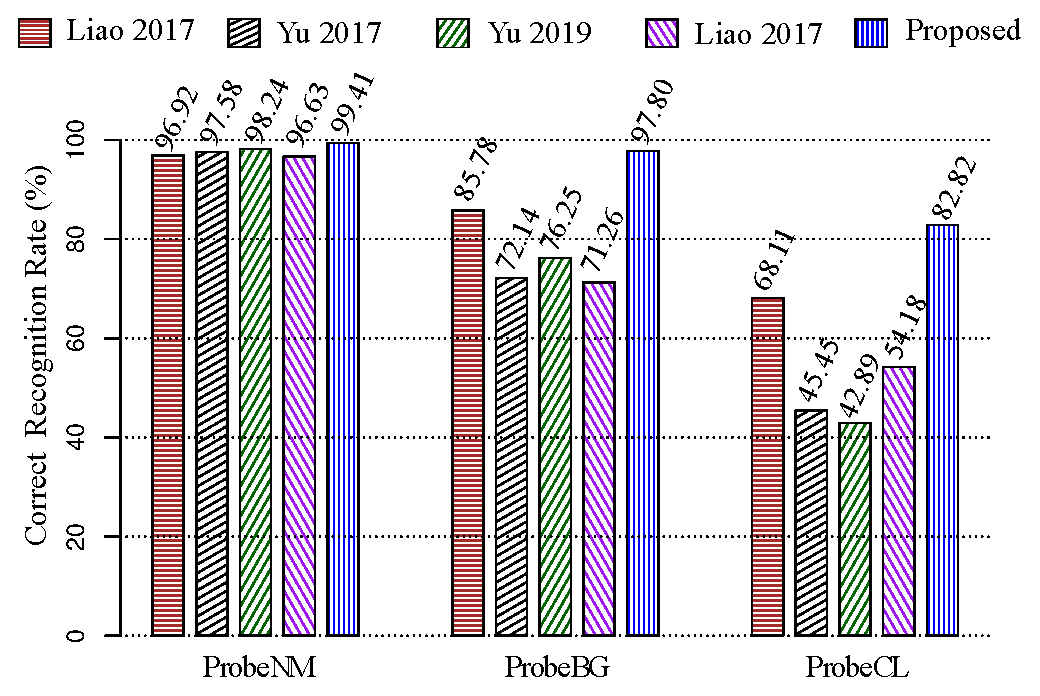
\includegraphics[width = 0.8\textwidth]{figures/comp_casia_b_without_view.eps}
	\caption [Correct class recognition rates (\%) of the proposed method with other state-of-the-art methods on all three probe set of CASIA B dataset without view variation] 
	{Correct class recognition rates (\%) of the proposed method with other state-of-the-art methods on all three probe set of CASIA B dataset without view variation. Proposed method demonstrates better performance compared to other by achieving $89.64\%$ and $96.45\%$ in two covariate conditions \textit{ProbeCL}, and \textit{ProbeBG} of CASIA B dataset respectively. The result proves the robustness of the proposed temporal network against carrying and clothing conditions variation.  \label{fig:comp_casia_b_without_view}
	}
\end{figure}


\subsubsection{Results on Single-View Gait Recognition of CASIA B Dataset with View Variation}
The performance of the proposed method on single-view gait recognition with view variation is demonstrated on Table~\ref{table:result_casia_b_with_view}. Here, for a specific gallery ($ \theta_g $) angle the average CCR (\%) of all eleven probe angles has been reported; our method achieved average CCR of $62.69\%$, $47.23\%$, and $33.46\%$ for \textit{ProbeNM}, \textit{ProbeBG}, and \textit{ProbeCL} respectively.


\begin{table}[t]
	\centering
	\caption{The average recognition rates for all three probe sets of CASIA B dataset. Each row represents the average value of all eleven probe angles at a specific gallery angle ($ \theta_g $) in all three probe sets. \label{table:result_casia_b_with_view}}
	{\begin{tabular*}{22pc}{cccc}\hline
			Gallery Angle &\textit{ProbeNM} &\textit{ProbeBG} &\textit{ProbeCL} \\\hline\noalign{\smallskip}
			${0^{\circ}}$	&61.73  &45.01  &32.40 \\\noalign{\smallskip}
			${18^{\circ}}$  &63.64  &47.80  &32.99 \\\noalign{\smallskip}
			${36^{\circ}}$	&67.30  &48.97  &34.46 \\\noalign{\smallskip}
			${54^{\circ}}$	&68.33  &50.15  &37.24 \\\noalign{\smallskip}
			${72^{\circ}}$	&68.33  &50.44  &39.0  \\\noalign{\smallskip}
			${90^{\circ}}$	&66.42  &49.12  &36.36  \\\noalign{\smallskip}
			${108^{\circ}}$ &64.22  &48.39  &34.75  \\\noalign{\smallskip}
			${126^{\circ}}$ &62.02  &47.07  &32.40  \\\noalign{\smallskip}
			${144^{\circ}}$ &58.80  &47.51  &31.82  \\\noalign{\smallskip}
			${162^{\circ}}$	&56.45  &44.13  &29.77  \\\noalign{\smallskip}
			${180^{\circ}}$ &52.35  &40.91  &26.83  \\\noalign{\smallskip}
			Mean &\textbf{62.69}  &\textbf{47.23} &\textbf{33.46} \\\hline
			
	\end{tabular*}}{}
\end{table}



\subsubsection{Comparison on Single-View Gait Recognition of CASIA B Dataset with State-of-the-art Methods with View Variation}
To better illustrate the robustness of our gait recognition method to view variation, the proposed method has been compared to three other state-of-the-art methods such as GaitGANv2~\cite{Yu_19}, PoseGait~\cite{Liao_19}, and Yu \textit{et al.}~\cite{Yu_17_spae}.  It has been observed from the Figure~\ref{fig:comp_casia_b_with_view} and Table~\ref{table:comp_casia_b_with_view} that the proposed method outperforms other in two covariate condition and achieves comparable performance in normal walking. 

Since, to recognize gait, we consider features based on the effective body joints, our method does not get affected by the variation in covariate conditions compared to other appearance-based method or model-based methods which consider ineffective features to build their gait descriptors. That's why our method is proven to be less sensitive to view angle variation and performs better in carrying bag and clothing condition. 

\begin{table}
	\centering
	\caption [Comparison among different state-of-the-art methods for gait recognition with view variation in all three probe sets of CASIA B dataset]
	{Comparison among different state-of-the-art methods for gait recognition with view variation in all three probe sets of CASIA B dataset. Here, each row represents the average value of all the gallery view's average recognition rate. It has been seen that, similar to first experiment, the proposed method achieves higher performance in two different probe set (\textit{ProbeBG}, \textit{ProbeCL}) and comparable performance in normal walking with other prevailing methods. \label{table:comp_casia_b_with_view}}
		
	{\begin{tabular*}{22pc}{cccc}\hline
				
				Methods &\textit{ProbeNM} &\textit{ProbeBG} &\textit{ProbeCL}\\
				\hline
				
				\noalign{\smallskip}
				Yu \textit{et al.}~\cite{Yu_17_spae} &62.82 &40.38 &26.05 \\ 
				
				
				\noalign{\smallskip}
				Yu \textit{et al.}~\cite{Yu_19} &66.34  &46.17  &25.91  \\
				
				\noalign{\smallskip}
				Liao \textit{et al.}~\cite{Liao_19}  &63.78  &42.52  &31.98  \\
				
				\noalign{\smallskip}
				Proposed &\textbf{62.69} &\textbf{47.23} &\textbf{33.46}\\
				\hline
\end{tabular*}}{}
\end{table}

\begin{figure}
	\centering
	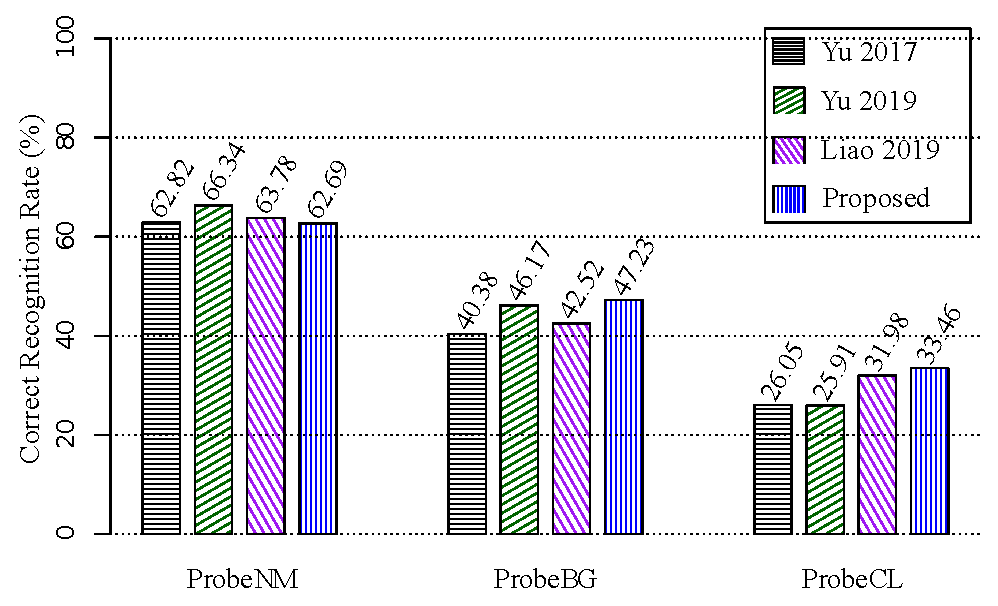
\includegraphics[width = 0.8\textwidth]{figures/comp_casia_b_with_view.eps}
	\caption [Comparison with different state-of-the-art algorithms for gait recognition with view variation in all three probe set of CASIA B dataset]
	{Comparison with different state-of-the-art algorithms for gait recognition with view variation in all three probe set of CASIA B dataset. Here, the value reported for each algorithm is the average of all of the gallery view's average \gls{ccr}. From the comparison, it is seen that our method outperforms other state-of-the-art methods by achieving $47.23\%$ and $33.46\%$ averaged accuracy in two covariate conditions \textit{ProbeBG}, and \textit{ProbeCL} respectively.   \label{fig:comp_casia_b_with_view}
	}
	
\end{figure}




%---------------------------------------------------------------------------------------------- 
\section{Cross-View Gait Recognition} \label{sec:cross_view}
The gait recognition scheme in which gallery and probe set are getting matched from two different views is commonly known as cross-view gait recognition. In this section we are going evaluate the performance of our proposed method on cross-view gait recognition. 
 


\begin{table}
	\centering
	\caption[Comparison of our proposed method with the previous best results of cross-view gait recognition ]
	{Comparison of our proposed method with the previous best results of cross-view gait recognition at different probe angles of CASIA B dataset by \gls{ccr}(\%). The network was trained according to experimental setup B to have the same setup with other methods. \label{table:comp_casia_b_cross_view}}
	
	{\begin{tabular*}{29pc}{c|c|cccc}\hline  \rule{0pt}{2ex}
	Probe View &Gallery View &CNN &CMCC &GEI-SVR  &\textbf{Proposed} \\ \hline\rule{0pt}{3ex}
	
	% first gallery angle
	\multirow{2}{*}{$0^{\circ}$} &$18^{\circ}$ &95.0 &85.0 &84.0 &\textbf{97.0} \\\rule{0pt}{2ex}
	
					&$36^{\circ}$ &73.5 &47.0 &45.0 &\textbf{80.0} \\ \hline\rule{0pt}{3ex}
	
	
	% second gallery angle
	\multirow{4}{*}{$54^{\circ}$} &$18^{\circ}$ &\textbf{91.5} &65.0 &64.0  &83.0 \\\rule{0pt}{2ex}
	
			&$36^{\circ}$ &98.5 &97.0 &95.0 &\textbf{100.0} \\\rule{0pt}{2ex}
	
			&$72^{\circ}$ &98.5 &95.0 &93.0 &\textbf{100.0} \\\rule{0pt}{2ex}
	
			&$90^{\circ}$ &\textbf{93.0} &63.0 &59.0 &83.0 \\\hline\rule{0pt}{3ex}
	
	
	% third gallery angle
	\multirow{4}{*}{$90^{\circ}$} &$54^{\circ}$ &-- &66.0 &63.0 &\textbf{84.0 }\\\rule{0pt}{2ex}
	
		&$72^{\circ}$ &\textbf{99.5} &96.0 &95.0 &96.0 \\ \rule{0pt}{2ex}
	
		&$108^{\circ}$ &\textbf{99.5} &95.0 &95.0 &95.0 \\ \rule{0pt}{2ex}
	
		&$126^{\circ}$ &-- &68.0 &65.0 &\textbf{71.0} \\\hline\rule{0pt}{3ex}
	
	
	% four gallery angle
	\multirow{4}{*}{$126^{\circ}$} &$90^{\circ}$ &\textbf{92.0} &78.0 &78.0 &76.0 \\\rule{0pt}{2ex}
			&$108^{\circ}$ &\textbf{99.0} &98.0 &98.0 &92.0 \\\rule{0pt}{2ex}
			&$144^{\circ}$ &97.0 &\textbf{98.0} &\textbf{98.0} &96.0 \\\rule{0pt}{2ex}
			&$162^{\circ}$ &\textbf{83.0} &75.0 &74.0 &77.0 \\\hline
	\end{tabular*}}{} 
\end{table}

\subsection{Comparison with the State-of-the-art Methods of CASIA B Dataset on Cross-View Gait Recognition}
To show the effectiveness of our proposed method in cross-view gait recognition, we make the comparison between the proposed method and three other state-of-the-art methods including CNN~\cite{Wu_17}, CMCC~\cite{Kusakunniran_14}, and GEI-SVR~\cite{Kusakunniran_10} with the same experimental setup. The probe angles were selected $0^{\circ}, 54^{\circ}, 90^{\circ}$, and $126^{\circ}$ for comparison. 

Although the proposed method contains only one model to handle any view angle variation, it achieves comparable performance with other prevailing state-of-the-art methods proposed in literature which were specially designed and trained for cross-view gait recognition. From Table~\ref{table:comp_casia_b_cross_view}, it is seen that CNN~\cite{Wu_17} achieves the highest recognition rates when the view variation is large due to the use of supervised information of all gallery angles during training.

The comparison in Table~\ref{table:comp_casia_b_cross_view} also illustrates that the proposed method performs better when the view variation is small. The reason for not achieving better performance at large view variation is because it was trained with only one view angle of the gallery. 



%---------------------------------------------------------------------------------------------- 
\section{Multi-View Gait Recognition} \label{sec:multi_view}
In multi-view gait recognition, multiple views of gallery gaits are combined to recognize an unknown gait view. For multi-view gait recognition, we initially identify the walking direction of a gait video using a 3D-CNN network. 

In our experiment, we evaluated the proposed 3D-CNN network with all three probe sets of CASIA B dataset and have achieved \textbf{100\%} identification accuracy. The experimental results proved the fact that our 3D-CNN is efficient in classifying the view angle from gait videos. Table~\ref{table:result_wd_identification} illustrates our test result. 

\begin{table}[t]
	\centering
	\caption[View angle identification rate (\%) of the proposed 3D-CNN network on CASIA B dataset]
	{View angle identification rate (\%) of the proposed 3D-CNN network on CASIA B dataset. The proposed view angle network successfully achieved \textbf{100\%} identification accuracy in all 11 view angles of all three probe sets in CASIA B dataset. \label{table:result_wd_identification}}
	
	{\begin{tabular*}{35pc}{cccc cccc cccc}\hline \noalign{\smallskip}
			View angle &${0^{\circ}}$	&${18^{\circ}}$  &${36^{\circ}}$ &${54^{\circ}}$	&${72^{\circ}}$	&${90^{\circ}}$	&${108^{\circ}}$ &${126^{\circ}}$ &${144^{\circ}}$ &${162^{\circ}}$  &${180^{\circ}}$ \\\hline \noalign{\smallskip}
			
			Rate(\%) &100 &100 &100 &100 &100 &100 &100 &100 &100 &100 &100 \\ \hline
	\end{tabular*}}{}
\end{table}


\begin{table}
	\centering
	\caption [Comparison with other state-of-the-art methods on all three probe set of CASIA B dataset in multi-view gait recognition]
	{Comparison with other state-of-the-art methods on all three probe set of CASIA B dataset in multi-view gait recognition. From the comparison, it is been observed that proposed two-stage network achieves higher average recognition rates in 8 of 11 different probe angles.\label{table:comp_multi_view}}
	\setlength{\tabcolsep}{3.5pt}
	\small
	{\begin{tabular*}{\textwidth}{|c|c|cccc cccc ccc|} \cline{1-13}\rule{0pt}{3ex}
		% header
		&Methods &${0^{\circ}}$ &${18^{\circ}}$  &${36^{\circ}}$ &${54^{\circ}}$ &${72^{\circ}}$	&${90^{\circ}}$	&${108^{\circ}}$ &${126^{\circ}}$ &${144^{\circ}}$ &${162^{\circ}}$  &${180^{\circ}}$ \\\cline{1-13}\rule{0pt}{3ex}
					
		% first probe set
		\multirow{4}{*}{\rotatebox{90}{Normal}} &Dupuis &97.2 &99.6 &97.2 &96.3 &98.8 &98.4 &97.1 &97.6 &97.14 &93.0 &96.0 \\\rule{0pt}{3ex}
		
		&VI-MGR &100.0 &99.0 &100.0 &99.0 &100.0 &100.0 &99.0 &99.0 &100.0 &100.0 &99.0 \\ \rule{0pt}{3ex}
		
		&Isaac &98.5 &99.0 &99.0 &97.0 &97.5 &96.0 &95.0 &97.5 &94.0 &93.9 &99.0 \\\rule{0pt}{3ex}
		
		&\textbf{Proposed} &100.0  &100.0  &100.0  &100.0  &100.0  &98.4  &100.0  &100.0  &100.0  &98.4  &96.8 \\\cline{1-13}\rule{0pt}{3ex}
	
	
	
		% second probe set
		\multirow{4}{*}{\rotatebox{90}{Bag}} &Dupuis &73.2 &74.1 &74.7 &76.3 &78.5 &75.8 &76.3 &76.7 &73.4 &73.2 &74.6 \\\rule{0pt}{3ex} 

		&VI-MGR &93.0 &89.0 &89.0 &90.0 &77.0 &80.0 &82.0 &84.0 &92.0 &93.0 &89.0 \\\rule{0pt}{3ex}

		&Isaac &95.0 &98.5 &96.5 &96.0 &97.5 &93.5 &93.5 &94.0 &92.5 &91.3 &94.4 \\\rule{0pt}{3ex}

		&\textbf{Proposed}  &100 &100 &100 &100 &98.39 &96.77 &96.77 &98.39 &98.39 &95.16 &91.93 \\\hline\rule{0pt}{3ex}


		% third probe set
		\multirow{4}{*}{\rotatebox{90}{Coat}} &Dupuis &81.64 &87.39 &86.29 &84.34 &89.96 &91.86 &89.50 &85.04 &72.24 &78.40 &82.70\\\rule{0pt}{3ex}
		
		&VI-MGR &67.0 &56.0 &70.0 &80.0 &71.0 &75.0 &77.0 &75.0 &65.0 &64.0 &66.0 \\\rule{0pt}{3ex}
		
		&Isaac &97.0 &99.5 &97.5 &94.0 &88.0 &90.5 &89.5 &94.5 &92.0 &91.3 &94.0 \\\rule{0pt}{3ex}
		
		&\textbf{Proposed} &81.52 &82.11 &83.58 &85.48 &84.46 &83.72 &83.28 &84.16 &83.58 &80.65 &78.45 \\\cline{1-13}
\end{tabular*}}{} 
\end{table}


%------------------------------------------------------------------------- 
\subsection{Comparison with the State-of-the-art Methods on Multi-View Gait Recognition}
To evaluate the performance of our proposed two-stage network, we compare it with the recent state-of-the-art multi-view gait recognition methods such as Dupuis~\textit{et al.}~\cite{Dupuis_13}, Isaac~\textit{et al.}~\cite{Isaac_17}, and VI-MGR~\cite{Choudhury_15} on all three probe set of CASIA B dataset. The comparison, as illustrated in Table~\ref{table:comp_multi_view} and Figure~\ref{fig:comp_casia_b_multi_view}, shows that the proposed method exceeds the previous best in result all three probe set by a significant margin. It outperforms other in total $ \textbf{8} $ of $ 11 $ view angles.

\begin{figure}
	\centering
	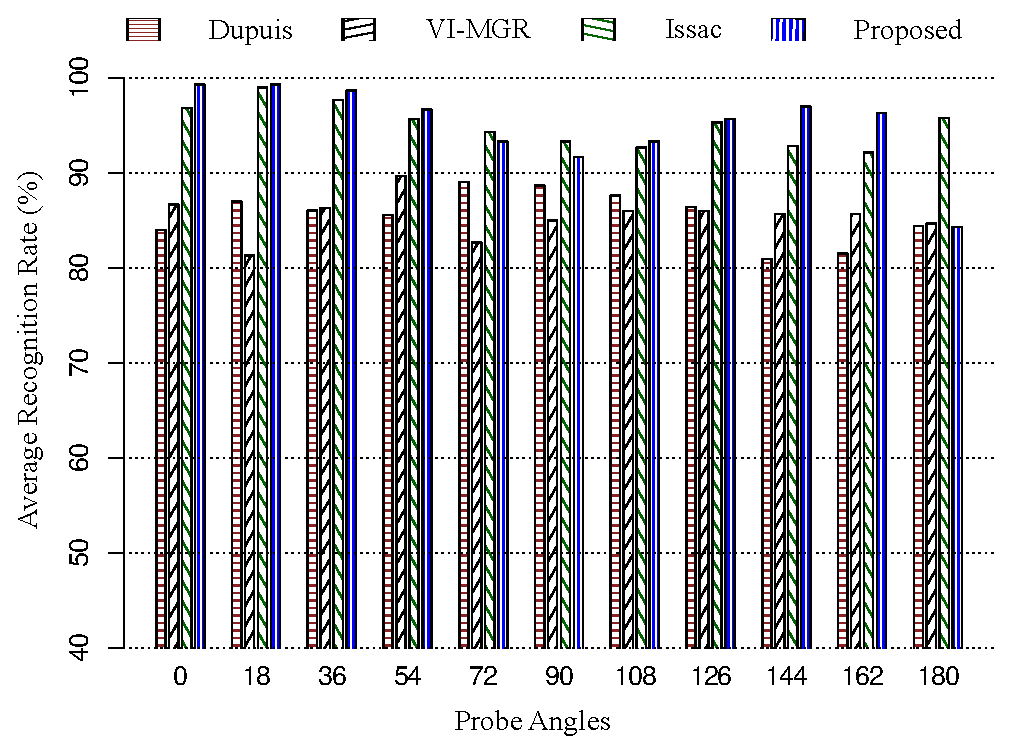
\includegraphics[width= 0.9\textwidth]{figures/comp_casia_b_multi_view.eps}
	\caption [Comparison on average recognition rates (\%) between the proposed method with other state-of-the-art methods in multi-view gait recognition]{
		Comparison on average recognition rates (\%) between the proposed method with other state-of-the-art methods in multi-view gait recognition. Our method achieves higher average recognition accuracy on \textbf{8 } of total 11 view angles of CASIA B dataset. \label{fig:comp_casia_b_multi_view}
	}

\end{figure}

